%% -*- TeX -*- -*- FR -*-
%V3.1 (révision le 26/11/2012 par B. Pinaud <bruno.pinaud@labri.fr>)
\documentclass[a4paper,pagenum,hyperref]{rnti}


%% commande pour guide de description de commandes
 \newcommand{\bs}{\symbol{'134}}% print backslash
 \newcommand{\Com}[1]{\texttt{\bs#1}\index{#1@\texttt{\bs#1}}}
 \newcommand{\Opt}[1]{\texttt{#1}\index{#1@\texttt{#1} option}}
 \newcommand{\File}[1]{\textit{#1}\index{#1@\textit{#1}}}
 \newcommand\rnti{\textit{rnti}}

 \usepackage{graphicx}
%packages nécessaires pour écrire des articles en français en utilisant les accents non latex.
\usepackage[T1]{fontenc}
\usepackage[latin1]{inputenc}

%pour bien présenter les URL et autres adresses emails
\usepackage{url}

 \domaine{G}

 \titrecourt{Guide utilisation de \textit{rnti.cls} v3}
 \nomcourt  {G. Ritschard}

 \titre     {%
    Guide d'utilisation de la classe \textit{rnti} version 3.1 pour
    articles de la
    Revue des Nouvelles Technologies de l'Information%
 }

 \auteur    {Gilbert Ritschard}

 \affiliation{%
    D\'{e}partement d'\'{e}conom\'{e}trie, Universit\'{e} de Gen\`{e}ve\\
    gilbert.ritschard@themes.unige.ch\\
    \href{http://www.antsearch.univ-tours.fr/rnti/}%
         {\http{http://www.antsearch.univ-tours.fr/rnti/}}%
 }

 \resume{
Ce guide de l'utilisateur de la classe \LaTeX\ \textit{rnti.cls}
version 3 d\'{e}crit l'installation de la classe ainsi que les options
et commandes qu'elle offre pour la production d'articles respectant
les normes de la \textit{Revue des Nouvelles Technologies de
l'Information} (RNTI). Il d\'{e}crit \'{e}galement l'usage du style
bibliographique \textit{rnti.bst} qui l'accompagne.
 }

 \summary{
This user guide of the \LaTeX\ class  \textit{rnti.cls} version 3
describes the installation of the class as well as the options and
commands provided to help formatting articles for the \textit{Revue
des Nouvelles Technologies de l'Information} (RNTI). It describes
also the accompagnying bibliographic style \textit{rnti.bst}.
 }

 \usepackage{color}
 \definecolor{dark-blue}{rgb}{0,0,.35}
 \definecolor{dark-red}{rgb}{0.35,0,.35}
 \definecolor{dark-green}{rgb}{0,0.35,0}

 \hypersetup{
 %ps2pdf=true,
 %urlcolor=black,%dark-blue, %magenta,
 filecolor=dark-green, %red,
 %linkcolor=dark-blue, % blue,
 %menucolor=white,
 citecolor=dark-red, % green,
 colorlinks=true,
 %a4paper=false,
 %bookmarksnumbered=false,
 %pdfpagemode=none,
 %plainpages=true,
 %pageanchor=false,
 %linktocpage=true,
 %pdfpagetransition=empty,
 %bookmarksopen=false,
 %backref=true
 }

 \setcounter{topnumber}{4}          % \setcounter{topnumber}{2}
 \def\topfraction{1}                % \def\topfraction{.7}
 \setcounter{bottomnumber}{2}       % \setcounter{bottomnumber}{1}
 \def\bottomfraction{1}             % \def\bottomfraction{.3}
 \setcounter{totalnumber}{5}        % \setcounter{totalnumber}{3}
 \def\textfraction{0}               % \def\textfraction{.2}
 \def\floatpagefraction{1}          % \def\floatpagefraction{.5}


%\usepackage{RNTIbiblio}

%%%%%%%%%%%%%%%%%%%%%%%%%%%%%%%%%%%%%%%%%%%%
\begin{document}

\section{Introduction}

La classe a \rnti\ a \'{e}t\'{e} con\c{c}ue pour faciliter la mise en forme
d'articles pour la revue RNTI. Des commandes simples sont propos\'{e}es
pour d\'{e}finir le titre, la liste des auteurs, leurs affiliations, le
r\'{e}sum\'{e} en fran\c{c}ais ainsi que le r\'{e}sum\'{e} (summary) en anglais.  Toutes
ces commandes doivent \^{e}tre utilis\'{e}es dans le pr\'{e}ambule, soit avant
le \verb|\begin{document}|, cette derni\`{e}re d\'{e}clenchant ensuite
automatiquement la mise en forme des informations fournies. La liste
compl\`{e}te des commandes propos\'{e}es et leur description sont donn\'{e}es \`{a}
la section~\ref{sec_commandes}.

Plusieurs options permettent par ailleurs de contr\^{o}ler diff\'{e}rents
aspects, comme la langue de l'article et l'impression des num\'{e}ros de
pages. Les options sont d\'{e}crites \`{a} la section~\ref{sec_options}.

La classe d\'{e}finit automatiquement diff\'{e}rents \'{e}l\'{e}ments du formatage
(dimension et positionnement de la page, police, forme des l\'{e}gendes
des tableaux et figures, \ldots).

Un style bibliographique \File{rnti.bst} est \'{e}galement propos\'{e} pour
g\'{e}n\'{e}rer les r\'{e}f\'{e}rences bibliographiques dans la forme demand\'{e}e \`{a}
partir de bases bibliographiques {\textsc{Bib}\TeX}. Pour les
citations, la classe reprend les r\`{e}gles de l'extension \File{natbib}
qui sont bri\`{e}vement d\'{e}crites \`{a} la section~\ref{sec_biblio}.

Cette description a \'{e}t\'{e} r\'{e}alis\'{e}e avec la classe \textit{rnti}. Les
hyperliens ont \'{e}t\'{e} obtenus avec l'option \Opt{hyperref} qu'il ne
faut \'{e}videmment pas utiliser pour les articles \`{a} publier.


 \section{Installation et utilisation\label{sec_installation}
        \index{installation}\index{utilisation}}

La distribution de la classe \rnti\ comprend les fichiers
 \begin{quote}
 \begin{tabular}{ll}
    \File{rnti.cls}   &  la classe \\
    \File{rnti.bst}   &  le style bibliographique\\
    \File{RNTI\_guide\_utilisateur.pdf}   &  ce manuel en format pdf\\
    \File{RNTI\_exemple.tex}  & le source d'un exemple d'article\\
    \File{RNTI\_exemple.pdf}  & le r\'{e}sultat de l'exemple\\
    \File{fg\_complex.pdf,.eps}     & figure utilis\'{e}e par l'exemple\\
    \File{biblio\_exemple.bib} & un exemple de fichier .bib\\
 \end{tabular}
 \end{quote}
L'exemple de fichier bibliographique contient notamment les
r\'{e}f\'{e}rences de ce guide et de l'exemple d'article.


Pour utiliser la classe \rnti, il convient de placer le fichier
\File{rnti.cls} \`{a} un endroit accessible \`{a} \LaTeX. La classe est
activ\'{e}e par la commande
%
 \begin{quote}
  \verb|\documentclass[a4paper,pagenum]{rnti}|
 \end{quote}
%
Les options, dont celles utilis\'{e}es ici ne sont que des exemples,
sont d\'{e}crites au point \ref{sec_options}.

La classe \rnti\ fait appel aux classes et extensions standard
suivantes qui doivent donc \^{e}tre disponibles dans votre environnement
\LaTeXe:
%
 \begin{quote}
        \textit{article.sty},
        \textit{babel.sty},
        \textit{fontenc.sty},
        \textit{ifthen.sty},
        \textit{layout.sty},
        %\texttt{graphicx} (optionnel)
 \end{quote}
%
ainsi que les extensions suivantes que l'on trouve sur le
CTAN\index{CTAN}
(\href{http://www.ctan.org}{\http{http://www.ctan.org}}):
%
 \begin{quote}
    \textit{times.sty},
    \textit{fancyhdr.sty},
    \textit{natbib.sty}.
 \end{quote}
%% - times.sty
%% - fancyhdr.sty       for handling page headers and footers
%% - natbib.sty         for handling authoryear citations


L'extension \File{babel} est utilis\'{e}e pour passer des r\`{e}gles de
typographie de l'anglais aux r\`{e}gles du fran\c{c}ais, notamment pour ce
qui est de l'espacement avant et apr\`{e}s la ponctuation, les r\`{e}gles de
c\'{e}sure, les dates et les intitul\'{e}s.
   Pour un fonctionnement correct des r\`{e}gles de c\'{e}sure, il faut
imp\'{e}rativement utiliser un format \File{latex.fmt} comprenant les
mod\`{e}les de c\'{e}sures anglais et fran\c{c}ais. V\'{e}rifier que le fichier
\File{language.dat} utilis\'{e} par \File{babel} contient quelque chose
du type
%
    \begin{verbatim}
    % File    : language.dat
    % Purpose : specify which hyphenation patterns to load
    %           while running iniTeX
    english ushyphen.tex
    french  frhyph.tex
    \end{verbatim}
    \vspace{-2ex}
%
Le cas \'{e}ch\'{e}ant modifier le fichier et recr\'{e}er le format
\File{latex.fmt} en ex\'{e}cutant \textit{initex} sur \File{latex.ltx}.



\begin{figure}[bt]\small
  %\hrule\vspace{-2ex}
  \framebox[\linewidth]{\parbox[t][28\baselineskip][c]{.9\linewidth}{\mbox}}

  \vspace{-28\baselineskip}
  %\fbox{\usebox{\verbatimbox}}
  {
\begin{verbatim}
 \documentclass[a4paper]{rnti}

 \titre     {Titre de votre article}
 \auteur    {Pr\'{e}nom1 Nom1\affil{1},
             Pr\'{e}nom2 Nom2\affil{1}\affilsep\affil{2} et
             Pr\'{e}nom3 Nom3\affil{2}
 }
 \affiliation{
            \affil{1}Institut1, adresse1\\
            nom1@email.fr\\
            \http{http://www.pageweb.fr/}
            \\
            \affil{2}Institut2, adresse2\\
            {nom2,nom3}@email.fr
 }
 \titrecourt{Ceci est le titre pour l'ent\^{e}te des pages paires}
 \nomcourt  {Noms auteurs pour ent\^{e}te pages impaires}
 \resume    {Ceci est le r\'{e}sum\'{e} qui para\^{\i}tra sur la
            premi\`{e}re page.}
 \summary   {This is the absract to be printed on the last
            page.}

 \begin{document}       % fin du pr\'{e}ambule
 \section{Introduction} % d\'{e}but de l'article
 ...
 \end{document} \end{verbatim}
}
 %\vspace{-3ex}

 %\hrule
 \vspace{1ex}
 \caption{Exemple d'utilisation de la classe \rnti.}
 \label{fg_exemple_utilisation}
\end{figure}


\section{Exemple d'utilisation}
 \label{sec_exemple}\index{utilisation}

Nous donnons \`{a} la figure~\ref{fg_exemple_utilisation} un exemple
illustrant l'usage des commandes essentielles de la classe.


On note que toutes les commandes qui d\'{e}finissent l'ent\^{e}te de
l'article et le r\'{e}sum\'{e} sont utilis\'{e}es dans le pr\'{e}ambule. Ceci est
requis, puisque c'est la commande \texttt{{\bs}begin\{document\}}
qui d\'{e}clenche la g\'{e}n\'{e}ration de l'ent\^{e}te.

\section{Les commandes}\label{sec_commandes}
 \index{Commandes}

\subsection{Commandes de d\'{e}finition de l'ent\^{e}te}

 \begin{description}

    \item
    \Com{titre}\verb+{+\textit{titre de l'article}\verb+}+


    \item
    \Com{auteur}\verb+{+\textit{pr\'{e}noms et noms des auteurs}\verb+}+

Les diff\'{e}rents auteurs sont s\'{e}par\'{e}s par des virgules.
%, le dernier
%\'{e}tant s\'{e}par\'{e} du pr\'{e}c\'{e}dent par \guilo{}\textit{et}\guilf{}.

    \item
    \Com{affiliation}\verb+{+\textit{Instituts, lieux et adresses
    e-mail}\verb+}+

    Commencer une nouvelle ligne (avec \verb+\\+) pour chaque
    nouvelle affiliation. De m\^{e}me commencer une nouvelle ligne pour
    chaque adresse e-mail. (Voir l'exemple de la
section~\ref{sec_exemple}.)

    \item
    \Com{affil}\verb+{+$n$\verb+}+,\Com{affilsep}

Lorsque les auteurs n'ont pas tous la m\^{e}me affiliation, utiliser
\Com{affil}\verb+{+$n$\verb+}+ pour indiquer l'affiliation de chaque
auteur. La commande \Com{affil}\verb+{+$n$\verb+}+ doit \^{e}tre accol\'{e}e
aux noms des auteurs dont l'affiliation est la $n$-\`{e}me dans la liste
des affiliations. Faire pr\'{e}c\'{e}der (sans espaces) la $n$-\`{e}me
affiliation par cette m\^{e}me commande. Pour $n \leq 4$, la commande
produit $n$ \'{e}toiles \affil{1} en indice sup\'{e}rieur. Pour $5 \leq n
\leq 8$, elle produit $n-4$ signes \affil{5} en indice sup\'{e}rieur.\\
Lorsqu'on doit indiquer plusieurs affiliations pour un m\^{e}me auteur,
utiliser \Com{affilsep} comme s\'{e}parateur entre
\verb+\affil{+$n$\verb+}+ . (Voir le cas de l'auteur2 dans l'exemple
de la section~\ref{sec_exemple}.)

    \item
    \Com{titrecourt}\verb+{+\textit{titre court pour ent\^{e}te}\verb+}+

D\'{e}finit le titre court qui appara\^{\i}t dans l'ent\^{e}te\index{ent\^{e}tes} des
pages paires.

    \item
    \Com{nomcourt}\verb+{+\textit{nom auteur pour ent\^{e}te}\verb+}+

D\'{e}finit la liste d'auteurs utilis\'{e}e pour l'ent\^{e}te\index{ent\^{e}tes} des
pages impaires. Pour un auteur, donner les initiales des pr\'{e}noms
suivie du nom. Pour deux auteurs proc\'{e}der de m\^{e}me pour chaque auteur
s\'{e}par\'{e} par \guilo{}et\guilf{} (ou ``and'' si l'article est en
anglais). Pour plus de deux auteurs utiliser la forme initiale et
nom du premier auteur suivi de \guilo{}et al.\guilf{}, par exemple
\guilo{}L. Breiman et al.\guilf{}.


    \item
    \Com{resume}\verb+{+\textit{texte du r\'{e}sum\'{e}}\verb+}+

Si l'article est en fran\c{c}ais, donner le r\'{e}sum\'{e} en fran\c{c}ais. Si
l'article est en anglais, donner le r\'{e}sum\'{e} en anglais. Le texte
donn\'{e} ici appara\^{\i}tra en d\'{e}but d'article sous le titre
\guilo{}R\'{e}sum\'{e}\guilf{} ou \guilo{}Abstract\guilf{} selon la langue
de l'article. (Pour fixer la langue, voir l'option \Opt{english} \`{a}
la section~\ref{sec_options}.) Pour supprimer le r\'{e}sum\'{e} (dans le cas
de papiers de deux pages ou moins), utiliser l'option
\Opt{noresume}.

    \item
    \Com{summary}\verb+{+\textit{text of the abstract}\verb+}+

Si l'article est en fran\c{c}ais, donner le r\'{e}sum\'{e} anglais. Si l'article
est en anglais, donner le r\'{e}sum\'{e} fran\c{c}ais. Ce texte appara\^{\i}tra en
fin d'article sous le titre \guilo{}Summary\guilf{} si l'article est
en fran\c{c}ais, et \guilo{}R\'{e}sum\'{e}\guilf{} s'il est en anglais.
 \end{description}

\subsection{Autres commandes}

  \begin{description}
    \item
    \Com{aftersummary}\verb+{+\textit{texte ou commandes \LaTeX}\verb+}+

A utiliser dans le cas exceptionnel o\`{u} l'on voudrait ajouter quelque
chose apr\`{e}s le \guilo{}Summary\guilf{}. Pour produire ce guide nous
l'avons par exemple utilis\'{e} pour placer l'index en fin de document.

    \item
    \Com{domaine}\verb+{+\textit{lettre majuscule}\verb+}+

S'utilise pour pr\'{e}ciser la lettre majuscule A (apprentissage), C
(classification), E (extraction des connaissances), S (statistique)
... de la s\'{e}rie RNTI qui doit figurer dans le pieds de
page\index{pieds de page}. La valeur par d\'{e}faut est X.  A utiliser
conjointement avec l'une des options \Opt{footer} ou \Opt{pagenum}.
Pour ce guide nous avons utilis\'{e} l'option \Opt{pagenum} et la
commande \verb+\domaine{G}+ pour produire \guilo{}RNTI - G -
\textit{page}\guilf{}.

    \item
    \Com{Eng},\Com{Fr}

Ces commandes changent les r\`{e}gles de typographie et de c\'{e}sure
respectivement vers l'anglais et le fran\c{c}ais, et d\'{e}finissent
certains intitul\'{e}s conform\'{e}ment \`{a} la langue. Elles sont par exemple
utiles dans les r\'{e}f\'{e}rences lorsque certaines sont en fran\c{c}ais et
d'autres en anglais. La section~\ref{sec_biblio} explique comment
utiliser ces commandes avec le style bibliographique
\File{rnti.bst}.

    \item
    \Com{guilo},\Com{guilf}

Pour les guillemets fran\c{c}ais nous recommandons ces commandes qui
introduisent automatiquement un petit espace avec le texte entre
guillemets. Par exemple \guilo{}texte\guilf{} est produit par
\verb+\guilo{}texte\guilf{}+.

    \item
    \Com{http}\verb+{+\textit{adresse internet}\verb+}+

Cette commande est fournie pour \'{e}viter l'espace qui est introduit
automatiquement par \File{babel} avant le \http{`:'} lorsque le
fran\c{c}ais est activ\'{e}.


  \end{description}

\section{Les options}\label{sec_options}
 \index{options}

 \begin{description}
%  \item
%  \Opt{altdash}
%
%Sur certain syst\`{e}me le tirait moyen \texttt{--} utilis\'{e} pour les
%l\'{e}gendes des tableaux et figures ne produit pas l'effet escompt\'{e}. En
%cas de probl\`{e}me activer l'option \Opt{altdash}.

  \item
  \Opt{english}, \Opt{french}

Indique la langue\index{langue} du texte. Par d\'{e}faut l'option
\Opt{french} est utilis\'{e}e. En activant l'option \Opt{english}, on
active les r\`{e}gles de typographie anglaise (ponctuation et c\'{e}sures)
ainsi que quelques intitul\'{e}s (``References'' au lieu de
``R\'{e}f\'{e}rences'', ``and'' au lieu de ``et'' dans les citations, etc.).
Sur la premi\`{e}re page on aura ``Abstract'' au lieu de ``R\'{e}sum\'{e}'', et
en fin de document ``R\'{e}sum\'{e}'' au lieu de ``Summary''. Voir \'{e}galement
les commandes \Com{Eng} et \Com{Fr}.

  \item\Opt{footer}, \Opt{pagenum}
  \index{num\'{e}rotation des pages}\index{pieds de page}

Produit les pieds de page respectivement sans et avec num\'{e}rotation
des pages.

  \item\Opt{hyperref}

Active l'extension \File{hyperref} qui permet de g\'{e}n\'{e}rer des
hyperliens\index{hyperliens} en compilant avec pdf\LaTeX. Ne doit
pas \^{e}tre utilis\'{e} pour produire des articles \`{a} publier dans RNTI.

  \item\Opt{langdepand}

Lorsque cette option est activ\'{e}e, le \verb+\andname+ utilis\'{e} dans
les r\'{e}f\'{e}rences (voir section~\ref{sec_biblio}) est d\'{e}fini par les
commandes \Com{Fr} et \Com{Eng}. Sinon, c'est-\`{a}-dire par d\'{e}faut, il
est contr\^{o}l\'{e} par la langue de l'article, soit le fran\c{c}ais par d\'{e}faut
ou l'anglais si \Opt{english} est activ\'{e}.


  \item\Opt{nobabel}

Supprime le chargement de l'extension \File{babel}. La classe
\textit{rnti} active \textit{babel} avec la commande
\verb+\uspackage[english,frenchb]{babel}+. Au cas o\`{u} vous voudriez
utiliser d'autres options, supprimez le chargement automatique et
chargez \textit{babel} avec les options voulues dans votre
pr\'{e}ambule.

  \item\Opt{nonatbib}

Supprime le chargement de l'extension \File{natbib}, pour le cas o\`{u}
l'on souhaite utiliser autre chose ou l'activer apr\`{e}s-coup avec des
options sp\'{e}cifiques.

  \item
  \Opt{noresume}

Supprime le r\'{e}sum\'{e} du d\'{e}but. A utiliser par exemple pour les textes
courts d'une seule page (r\'{e}sum\'{e} de poster).


  \item
  \Opt{nosummary}

Supprime le r\'{e}sum\'{e} du d\'{e}but ainsi que celui dans l'autre langue de
la fin.


  \item\Opt{oldfancyhdr}

Pour ceux qui utilisent encore les vieilles versions de
\textit{fancyhdr}.

  \item\Opt{showlayout}

Produit en fin de document deux pages illustrant la mise en page et
les valeurs des param\`{e}tres de mise en page. Utilise l'extension
\File{layout.sty}. Cette option est utile pour r\'{e}gler si n\'{e}cessaire
des param\`{e}tres de mise en page.

  \item\Opt{submission}

Cette option doit \^{e}tre activ\'{e}e pour la soumission de papiers lorsqu'un texte anonyme est demand\'{e} pour le processus d'\'{e}valuation. L'option rend invisible les noms et affiliations des auteurs dans le titre de l'article ainsi que dans l'ent\^{e}te des pages impaires. Il appartient \`{a} l'auteur d'\'{e}liminer toute autre trace qui permettrait d'identifier les auteurs.



 \end{description}


\section{Pr\'{e}paration de la bibliographie et citations}\label{sec_biblio}
 \index{bibliographie, pr\'{e}paration}\index{citation}

 \begin{figure}[b]
{\small
  \framebox[\linewidth]{\parbox[t][22\baselineskip][c]{.9\linewidth}{\mbox}}

  \vspace{-22\baselineskip}
%
\begin{verbatim}
 \begin{bibliography}

 \bibitem[{Breiman et~al.}(1984){Breiman, Friedman, Olshen,
   \andnamec{} Stone}]{brei:frie:olsh:ston:1984}
 Breiman, L., J.~H. Friedman, R.~A. Olshen, \andname{} C.~J. Stone
 (1984).
 \newblock {\em Classification And Regression Trees}.
 \newblock New York: Chapman and Hall.

 \bibitem[{Quinlan}(1986){Quinlan}]{quin:1986ID3}
 Quinlan, J.~R. (1986).
 \newblock Induction of decision trees.
 \newblock {\em Machine Learning\/}~{\em 1}, 81--106.

 \bibitem[{Quinlan}(1993){Quinlan}]{quin:1993}
 Quinlan, J.~R. (1993).
 \newblock {\em C4.5: Programs for Machine Learning}.
 \newblock San Mateo: Morgan Kaufmann.

 \end{bibliography}\end{verbatim}
}
 \caption{Exemples de {$\bs{\texttt{bibitem}}$}\enspace.}
 \label{fg_exemple_saisie_biblio}
 \end{figure}

La revue RNTI demande des citations sous forme auteur-ann\'{e}e. La
classe \rnti\ fait appel \`{a} cette fin \`{a} l'extension \File{natbib}.

\subsection{Utilisation de l'extension natbib.sty}

Pour un bon fonctionnement, les \verb+\bibitem+ doivent avoir la
forme suivante dans les r\'{e}f\'{e}rences:
%
 \begin{quote}
    \Com{bibitem}\verb+[+\textit{liste courte des
    auteurs}\verb+(+\textit{ann\'{e}e}\verb+)+\textit{liste longue des
    auteurs}\verb+]{+\textit{cl\'{e}}\verb+}+\\
    NomAuteur1, Initiale1 and Initiale2 NomAuteur2 and ...
    (\textit{ann\'{e}e})\\
    Titre, ...
 \end{quote}
%
la liste longue des auteurs \'{e}tant optionnelle. La
figure~\ref{fg_exemple_saisie_biblio} donne quelques exemples
d'entr\'{e}es dans la bibliographie. Les commandes \Com{andname} et
\Com{andnamec} utilis\'{e}es dans ces exemples sont d\'{e}finies par la
classe \rnti\ en fonction de la langue activ\'{e}e. Par d\'{e}faut
\verb+\andname+ et \verb+\andnamec+ sont d\'{e}finis tous deux comme
\guilo{}et\guilf{} pour un article en fran\c{c}ais (option \Opt{french}
activ\'{e}e par d\'{e}faut), ou comme \guilo{}and\guilf{} pour un article en
anglais (option \Opt{english}). Si l'on active l'option
\Opt{langdepand}, \verb+\andname+ est d\'{e}fini comme
\guilo{}et\guilf{} par \Com{Fr}, et comme \guilo{}and\guilf{} par
\Com{Eng}. L'option \Opt{langdepand} ne doit pas \^{e}tre utilis\'{e}e pour
les articles RNTI.

A la compilation, la classe \File{rnti} liste les r\'{e}f\'{e}rences avec un
espacement fix\'{e} par d\'{e}faut \`{a} \Com{bibsep}\verb+=.6ex+. On peut
\'{e}ventuellement changer cette valeur en pla\c{c}ant par exemple
\Com{bibsep}\verb+=.5ex+ avant les commandes produisant la
bibliographie.


 \begin{table}[htb]
 \begin{center}
    \begin{tabular}{ll}
    \hline\hline
     syntaxe & exemple d'output \\
     \hline
    \Com{citet}\verb+{+\emph{cl\'{e}}\verb+}+
          & \citet{brei:frie:olsh:ston:1984} \\
    \Com{citet}\verb+[+chapitre 4\verb+]{+\emph{cl\'{e}}\verb+}+
          & \citet[chapitre 4]{brei:frie:olsh:ston:1984}\\
    \Com{citep}\verb+{+\emph{cl\'{e}}\verb+}+
          & \citep{brei:frie:olsh:ston:1984} \\
    \Com{citep}\verb+[+voir\verb+][+chapitre 4\verb+]{+\emph{cl\'{e}}\verb+}+
          & \citep[voir][chapitre 4]{brei:frie:olsh:ston:1984}\\
    \Com{citet}\verb+{+\emph{cl\'{e}1,cl\'{e}2}\verb+}+
          & \citet{quin:1986ID3,quin:1993}\\
    \hline
    \end{tabular}
 \caption{Principales commandes de citation.}
 \label{tab_commandes_citation}
 \end{center}
 \end{table}

On utilise ensuite dans le texte l'une des commandes de
citation\index{citation} \'{e}num\'{e}r\'{e}es au
tableau~\ref{tab_commandes_citation}. Pour plus de d\'{e}tails et
d'autres variantes de citations, voir la description de l'extension
\textit{natbib} \citep{Daly:2003}.



\subsection{Le style bibliographique \textit{rnti.bst}}

Le plus simple pour g\'{e}n\'{e}rer la bibliographie sous la forme voulue
est de mettre les r\'{e}f\'{e}rences dans une base de donn\'{e}es
bibliographique \textsc{Bib}\TeX\ et d'utiliser le style
bibliographique \File{rnti.bst} en pla\c{c}ant les commandes
%
 \begin{quote}
 \Com{bibliographystyle}\verb+{rnti}+\\
 \Com{bibliography}\verb+{+\textit{maBaseBibliographique}\verb+}+
 \end{quote}
%
\`{a} l'endroit o\`{u} doit \^{e}tre plac\'{e}e la bibliographie, c'est-\`{a}-dire en
fin de document avant les \'{e}ventuelles annexes.

Pour la pr\'{e}paration de la base de donn\'{e}es bibliographiques on pourra
par exemple consulter \citet[][annexe B]{kopka:daly:1995}. Par
exemple, pour ce guide d'utilisation nous avons utilis\'{e} le fichier
\File{biblio\_exemple.bib} qui contient entre autres les entr\'{e}es de
la figure~\ref{fg_exemple_entrees_fichier_bib}.

 \begin{figure}[htb]
{\small
  \framebox[\linewidth]{\parbox[t][45\baselineskip][c]{.9\linewidth}{\mbox}}

  \vspace{-46\baselineskip}
%
 \begin{verbatim}
 @BOOK{brei:frie:olsh:ston:1984wads,
    Address        = {Belmont, CA},
    Author         = {Breiman, L. and J. H. Friedman and
                      R. A. Olshen and C. J. Stone},
    Publisher      = {Wadsworth International Group},
    Title          = {Classification And Regression Trees},
    Year           = {1984},
    Language       = {\Eng}
 }
 @ARTICLE{quin:1986ID3,
    Author         = {Quinlan, J. R.},
    Journal        = {Machine Learning},
    Pages          = {81-106},
    Title          = {Induction of Decision Trees},
    Volume         = {1},
    Year           = {1986},
    Language       = {\Eng}
 }
 @INCOLLECTION{malerba:appi:ceci:mono:2002,
    Author         = {Malerba, Donato and Annalisa Appice and
                      Michelangelo Ceci and Marianna Monopoli},
    Booktitle      = {Foundations of Intelligent Systems, {ISMIS}
                      2002},
    Editor         = {Mohand-Said Hacid and Zbigniew W. Ras and
                      Djamel A. Zighed and Yves Kodratoff},
    Pages          = {393-402},
    Publisher      = {Springer},
    Series         = {LNAI},
    Title          = {Trading-Off Local versus Global Effects
                      of Regression Nodes in Model Trees},
    Volume         = {2366},
    Year           = {2002},
    Language       = {\Eng}
 }
 @TECHREPORT{Daly:2003,
    Author         = {Daly, Patrick W.},
    Institution    = {CTAN (http://www.ctan.org/)},
    Note           = {Describes the package natbib},
    Title          = {Natural Sciences Citations and References
                      (Author--Year and Numerical Schemes)},
    Type           = {{\LaTeX} Package description},
    Year           = {2003},
    Language       = {\Eng}
 }\end{verbatim}
 }
 \caption{Exemple d'entr\'{e}es d'un fichier .bib.}
 \label{fg_exemple_entrees_fichier_bib}
 \end{figure}

Pour plus de d\'{e}tails, le lecteur peut examiner le contenu du fichier
\File{biblio\_exemple.bib}. L'utilitaire \File{BibTeXMng}
(\href{http://www.latexsoft.com/bibtexmng.htm}
{\http{http://www.latexsoft.com/bibtexmng.htm}}) pourra s'av\'{e}rer
utile pour les personnes peu famili\`{e}res avec la pr\'{e}paration de
telles bases bibliographiques.

Les exemples de \Com{bibitem} de la
figure~\ref{fg_exemple_saisie_biblio} ont \'{e}t\'{e} g\'{e}n\'{e}r\'{e}s
automatiquement par le style \File{rnti.bst} qui les place dans le
fichier \textit{nomdocument.bbl}.

\section{Tableaux et figures}

Les tableaux\index{tableaux} et les figures\index{figures} doivent
\^{e}tre plac\'{e}s dans les environnements flottants, soit
%
 \begin{quote}
 \verb+\begin{table}[htb]  ... \end{table} + pour les tableaux\\
 \verb+\begin{figure}[htb] ... \end{figure}+ pour les figures\\
 \end{quote}
%
Les l\'{e}gendes\index{l\'{e}gendes} sont donn\'{e}es avec la commande
\Com{caption}\verb+{+\textit{l\'{e}gende.}\verb+}+ qui doit \^{e}tre plac\'{e}e
dans l'environnement flottant \textit{apr\`{e}s} le tableau ou la
figure. Le texte de la l\'{e}gende doit se terminer avec un point.

Pour ins\'{e}rer les figures, nous recommandons l'usage de l'extension
\File{graphicx} et de la commande \Com{includegraphics}. La
figure~\ref{fg_complex} a par exemple \'{e}t\'{e} g\'{e}n\'{e}r\'{e}e avec les
instructions

{\small
 \begin{verbatim}
 \begin{figure}[htb]
  \center
  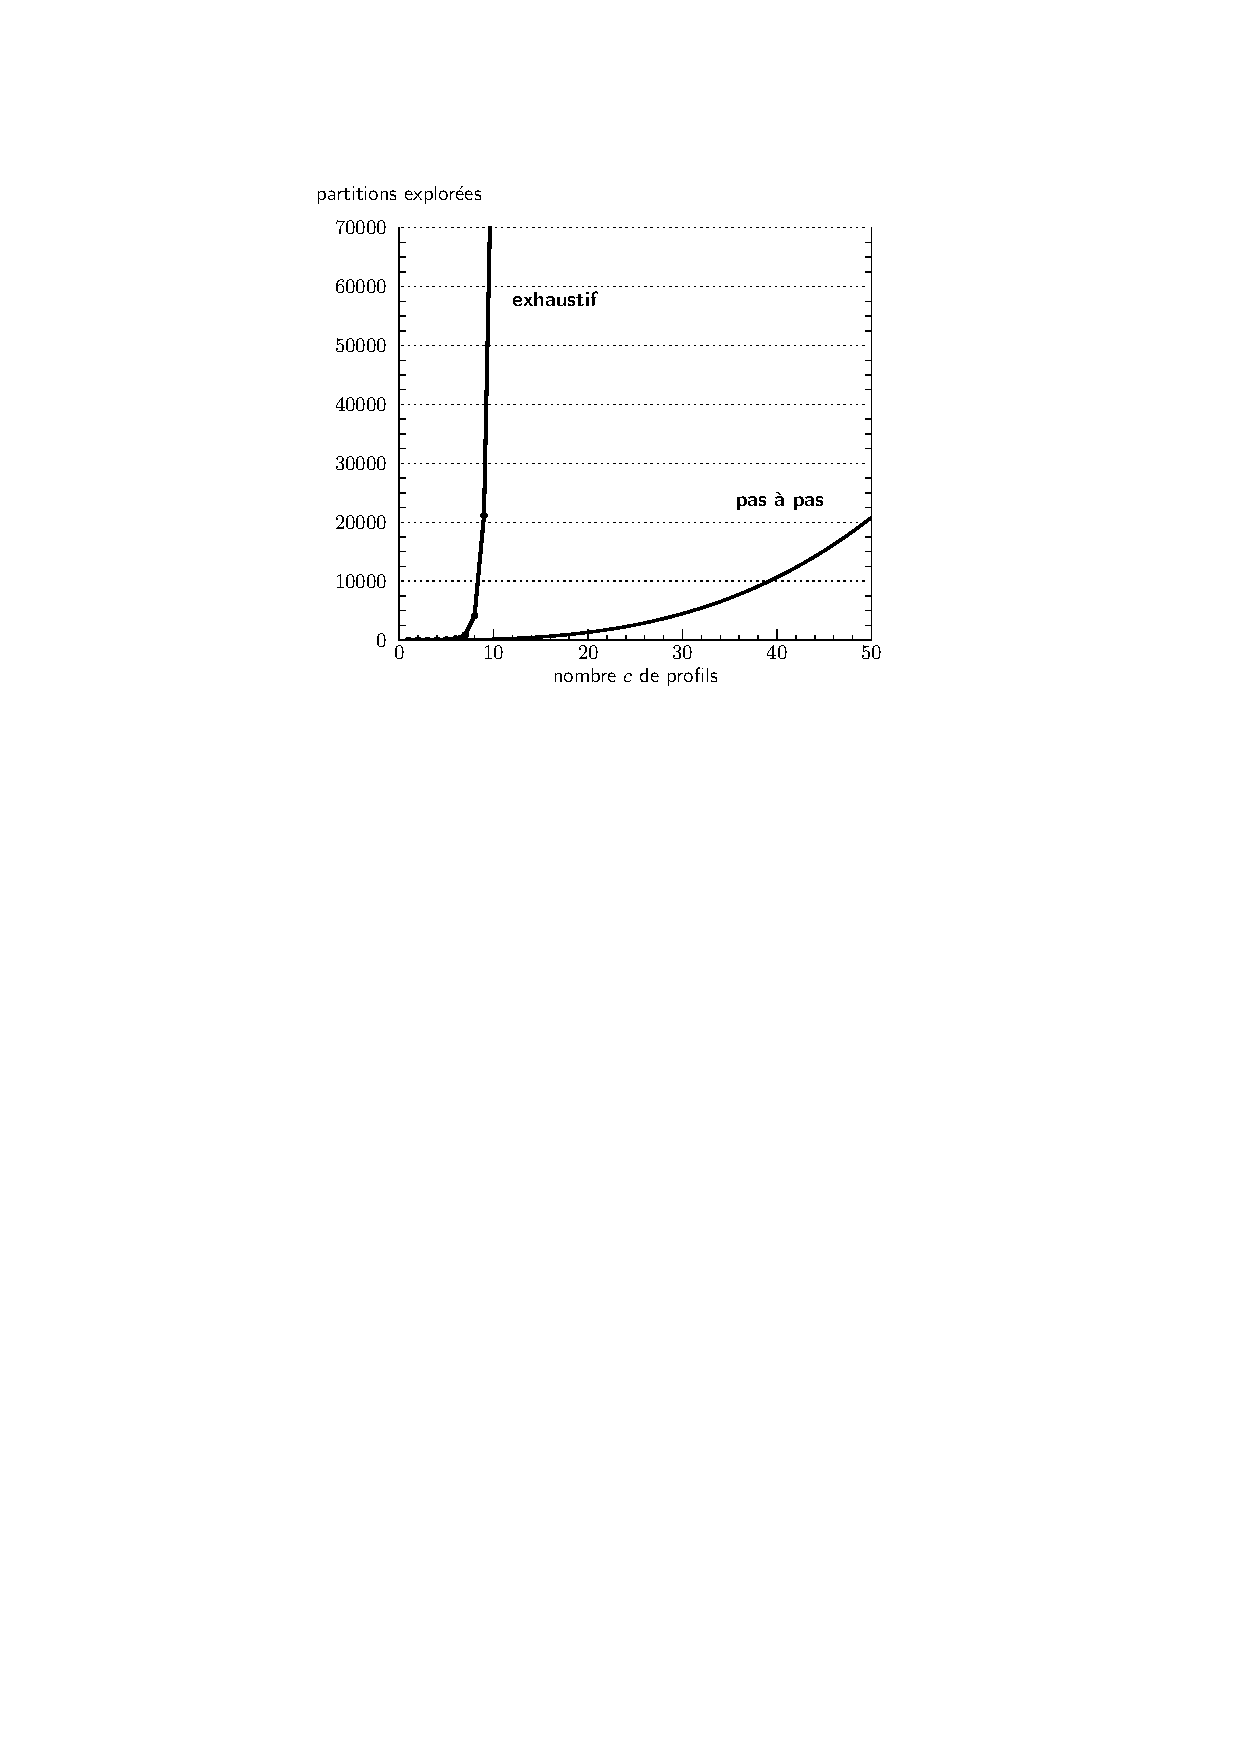
\includegraphics[width=.8\linewidth]{fg_complex}
 \caption{Exemple de figure.}
 \label{fg_complex}
 \end{figure}\end{verbatim}
 }

 \begin{figure}[htb]
  \center
  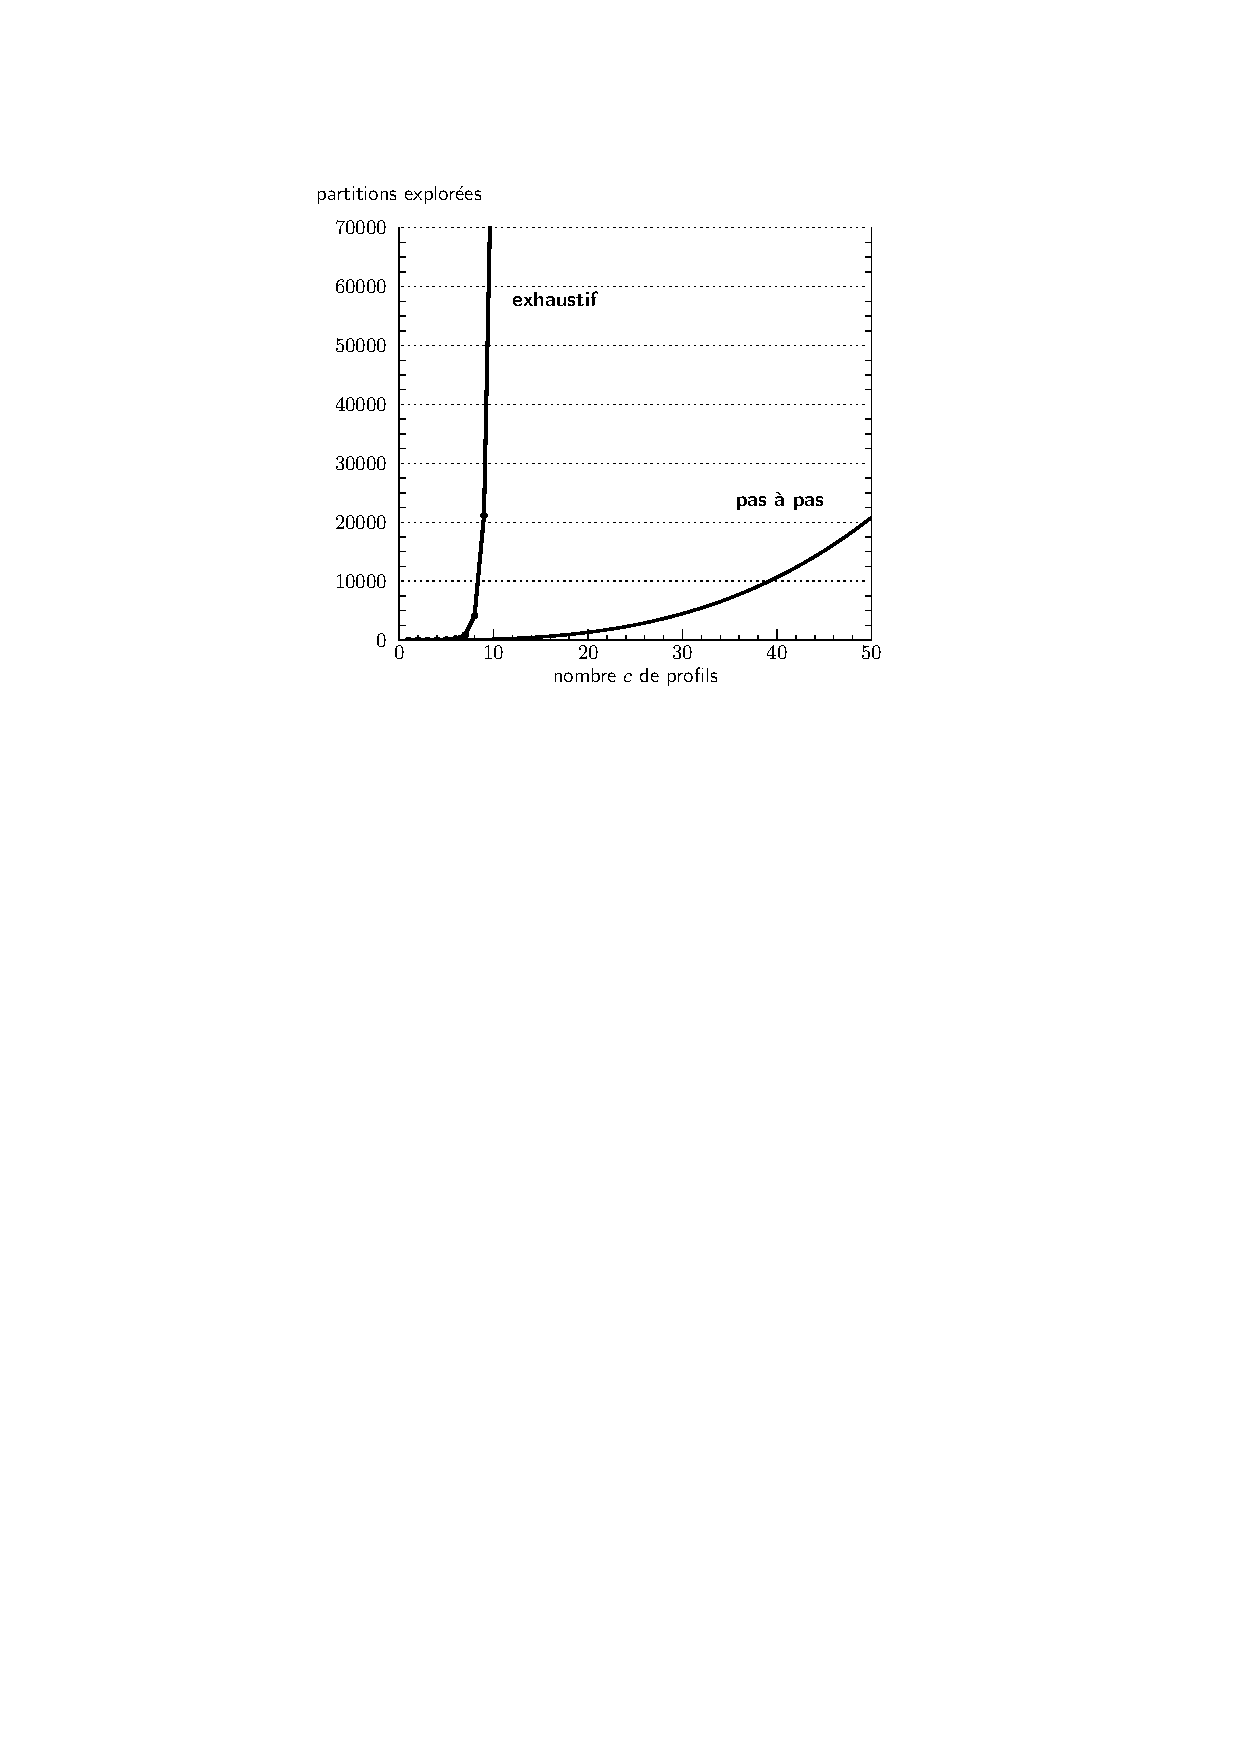
\includegraphics[width=.8\linewidth]{fg_complex}
 \caption{Exemple de figure.}
 \label{fg_complex}
 \end{figure}

Il est pr\'{e}f\'{e}rable de ne pas indiquer l'extension du nom de fichier
de la figure (\textit{fg\_complex} dans l'exemple ci-dessus). En
compilant le texte avec \LaTeX\, \verb+\includegraphics+ cherche
successivement le fichier avec une extension .eps ou .ps, tandis
qu'avec pdf\LaTeX\, la commande cherche une figure avec l'extension
.png, .pdf ou .jpg.
\bigskip

Pour les tableaux\index{tableaux}, nous recommandons d'\'{e}viter les
traits s\'{e}parateurs verticaux qui alourdissent la page. Le
tableau~\ref{tab_example_tableau} a par exemple \'{e}t\'{e} g\'{e}n\'{e}r\'{e} avec les
instructions suivantes:

{\small
 \begin{verbatim}
 \begin{table}[htb]
  \center\small
  \begin{tabular*}{\linewidth}{@{\extracolsep{\fill}}lccccccc}
  \hline\hline
        & $q$   & $c^*$ & $p$   & $n$   & $D(m_0|m)$ & $d$ & sig.\\
    \hline
    CHI & 12    & 263   & 299   & 5770  & 822.2      & 33  & .00 \\
    CHF & 10    & 644   & 674   & 35239 & 4293.3     & 27  & .00 \\
    CHG & 11    & 684   & 717   & 99641 & 16258.6    & 30  & .00 \\
    \hline
  \end{tabular*}
 \caption{Exemple de tableau.}
 \label{tab_example_tableau}
 \end{table}\end{verbatim}
 }



 \begin{table}[htb]
  \center\small
  \begin{tabular*}{\linewidth}{@{\extracolsep{\fill}}lccccccc}
  \hline\hline
        & $q$   & $c^*$ & $p$   & $n$   & $D(m_0|m)$ & $d$ & sig.\\
    \hline
    CHI & 12    & 263   & 299   & 5770  & 822.2      & 33  & .00 \\
    CHF & 10    & 644   & 674   & 35239 & 4293.3     & 27  & .00 \\
    CHG & 11    & 684   & 717   & 99641 & 16258.6    & 30  & .00 \\
    \hline
  \end{tabular*}
 \caption{Exemple de tableau.}
 \label{tab_example_tableau}
 \end{table}


\section{Les annexes}

Si du mat\'{e}riel doit \^{e}tre plac\'{e} en annexe\index{annexes}, celui-ci
sera plac\'{e} \textit{apr\`{e}s} la bibliographie dans une section
introduite avec les commandes
 \begin{quote}
  \verb+\appendix+
  \verb+\section*{Annexe}+
 \end{quote}
S'il y a plusieurs annexes, on les num\'{e}rotera : Annexe 1, Annexe 2,
etc.

\bigskip

\section{Conclusion}

L'objectif de ce guide et de la classe \rnti\ est de vous aider \`{a}
mettre en forme les articles. Si la forme est importante, le contenu
est lui essentiel, et l\`{a} il vous appartient d'en assurer le s\'{e}rieux,
l'originalit\'{e} et la rigueur scientifique. Bons articles!

%bibliographie au format bibtex
\bibliographystyle{rnti}
\bibliography{biblio_exemple}


\appendix
\section*{Annexe}

Voici un exemple d'annexe.


\end{document}
